\documentclass[10pt,letterpaper]{article}
\usepackage{cogsci}
\usepackage{pslatex}
\usepackage{apacite}
\usepackage{amsmath, amsfonts, amssymb}
\usepackage{graphicx}

\title{Toward a Theory of Timing Effects in Self-Organized Sentence Processing}
 
\author{{\large \bf Garrett Smith (garrett.smith@uconn.edu)} \\
  Department of Psychological Sciences, 406 Babbidge Road, Unit 1020\\
  Storrs, CT 06269 USA
  \AND {\large \bf Whitney Tabor (whitney.tabor@uconn.edu)} \\
  Department of Psychological Sciences, 406 Babbidge Road, Unit 1020\\
Storrs, CT 06269 USA}


\begin{document}
\maketitle

\begin{abstract}
Dynamical sentence processing models provide a natural explanation for ``grammar flouting'' interference effects in sentence comprehension and production, like local coherence effects, using bottom-up structure building that at least temporarily entertains ungrammatical structures. Since a major source of data on these and other phenomena comes from timing data (reading times and production latencies), it is important that such models be able to account for timing effects. However, previous dynamical parsing models have only limited coverage of reading time data, and more importantly, there is no unified theory of why different sentences should take different amounts of time to process in a dynamical parser. Here, we present the self-organized sentence processing (SOSP) framework, a dynamical sentence processing model in which the processing dynamics locally maximize a harmony function specifying the well-formedness of linguistic structures (modulo the effect of noise). We show that processing speed is inversely related to the harmony of the structure the parser chooses: higher-harmony structures (even ungrammatical ones) are processed faster than lower-harmony structures. We show that the system provides a mechanistic explanation for local coherence effects. The transparent mapping between linguistic structures and quantitative predictions about processing dynamics in SOSP will facilitate future comparisons with other well-established sentence frameworks like ACT-R and surprisal theory.

\textbf{Keywords:} sentence comprehension, local coherence effects, dynamical systems models, self-organization
\end{abstract}

\section{Introduction}
Most of the time, people produce and interpret sentences according to the rules of some grammar. However, they sometimes temporarily entertain or even settle on structures that are not completely faithful to those rules. Here, we introduce self-organizing sentence processing (SOSP) \cite{smith2018self} as a general theory of reading time effects that we then apply to an interesting case of ``grammar flouting'' interference in sentence comprehension.

We consider local coherence effects \cite{tabor2004effects, konieczny2005psychological, paape2015local, bicknell2009correcting, levy2009eye}, where the parser seems to entertain a locally coherent structure that is incompatible with the rest of the sentence. For example, \citeA{tabor2004effects} used sentences like \emph{The coach smiled at the player \textbf{tossed/thrown} the frisbee\dots}. The sequence \emph{the player tossed the frisbee\dots}, on its own, is a grammatical sentence. However, the rest of the sentence in which it appears rules out this structure, since the preposition \emph{at} cannot grammatically take a sentence as its complement (*[PP \emph{at} [S \emph{the player tossed the frisbee\dots}]]). Tabor and colleagues found that participants read the region containing \emph{tossed} significantly longer than the corresponding region for \emph{thrown}, suggesting that the locally coherent but globally illicit parse was competing with the correct parse ([PP \emph{at} [NP \emph{the} [N' \emph{player} [VP \emph{tossed the frisbee}]]]]). This result suggests that people at least temporarily entertain ungrammatical parses and motivates a theory of parsing in which suboptimal structures can influence processing (unlike strictly rational approaches to sentence processing, as argued in, e.g., \citeA{levy2009eye}).

\begin{figure}[h!]
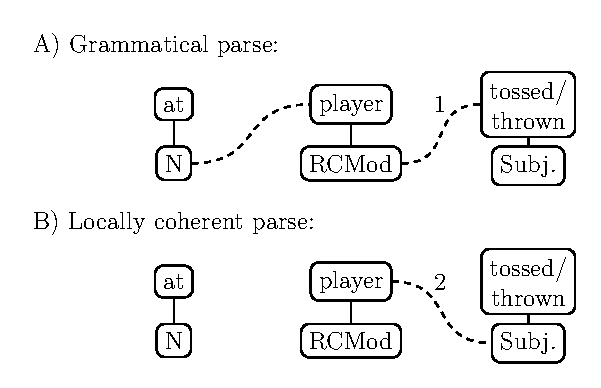
\includegraphics[width=\linewidth]{../Figures/LocalCoherenceStructs.pdf}
\caption{Dependency structures assumed to model \citeA{tabor2004effects}. Panel A shows the gramatical parse: The preposition \emph{at} takes \emph{player} as its nominal dependent, and \emph{player} takes the participle as the head of a relative clause modifier. Panel B shows the ungrammatical, locally coherent parse in which \emph{at} fails to attach anything as its dependent, and the participle takes \emph{player} as its subject dependent. The numbers on the links are used to label the links in the simulations below.}
\label{harmonylandscape}
\end{figure}

%The second example of grammar-flouting interference comes from studies of agreement attraction in comprehension. When asked to repeat a subject noun phrase and then complete the rest of the sentence, participants produce a verb that agrees in number with a noun other than the grammatical subject of the sentence, e.g., \emph{the key to the cabinets \textbf{are}\dots} \cite[among many others]{bock1991broken} in a small but reliable proportion of trials. In addition, \citeA{haskell2003conflicting} provided evidence that participants were slower to complete the sentence with a plural intervening noun (e.g., \emph{cabinets}) than with a singular (e.g., \emph{cabinet}). Together, the production and timing effects suggest that not only do participants temporarily entertain ungrammatical structures, they can sometimes stabilize on them long enough to actually produce them.

Our focus on timing effects here is motivated by the fact that previous dynamical parsers like SOSP have had little success in predicting timing data, despite the fact that time plays such a central role in these models---they are all implemented as sets of differential equations or iterated maps which describe how the state of a parse changes in time. The dynamical models of \citeA{kempen1989incremental, vosse2009unification, tabor2004evidence} derive some timing predictions for a handful of phenomena via direct simulations, however, a relatively large number of other models \cite{vandervelde2006neural, vosse2000syntactic, cho2016bifurcation, cho2017incremental, smith2018self, gerth2009unifying} either do not make timing predictions or the timing predictions are not discussed. More importantly, though, there is no theory of why processing one structure should take longer than another structure in these frameworks. In the SOSP framework we present, timing effects are shown to be directly related to the well-formedness (harmony) \cite{smolensky1986information} of the linguistic structure that is built: Sentence structures that are less well-formed take longer to process than more well-formed structures, and the overall average settling time (comparable to averages calculated from experiments) is average of the settling times to each parse chosen weighted by how frequently that parse is selected. While this result seems intuitive, we show below how it follows directly from the calculation of harmony and the dynamical equations that govern how the system parses. Moreover, it makes novel testable predictions that, to our knowledge, are unique among extant theories of sentence processing.

We note that one very promising related result is presented in \citeA{cho2018dynamic}, where Cho et al. show that, in a related but different dynamical parser (Gradient Symbolic Computation, GSC), the change in harmony from one parsing step to the next is equivalent to surprisal, which is known to predict reading times over a large range of word predictability \cite{hale2001probabilistic, levy2008expectation, smith2013effect}. This effort is closely related to the present paper, but it differs in that GSC only grammatical structures to stabilize by the end of a sentence. In SOSP, allowing the system to stabilize on ungrammatical structures will be key to explaining local coherence effects.

\section{Self-organized sentence processing}
%Harmony = consistency/coherency \cite{smolensky1986information}; processing is maximizing self-consistency of representation given input. Self-consistency given by harmony function $H$.

In SOSP, linguistic structures are built out of lexically anchored syntactic treelets. The treelets connect with each other via graded attachment links. We assume for simplicity a dependency grammar formalism \cite{hudson2007language, mcdonald2013universal}, so the only attachment sites are ones allowing a word to attach as the dependent of another word (\emph{head} attachment sites) and ones that allow other words to attach as dependents (\emph{dependent} attachment sites). The head and dependent attachment sites on each treelet are feature vectors encoding syntactic and semantic properties of a word and its expected dependents, respectively. Some features can change (e.g., the number marking on the determiner \emph{the} depends on the number of its licensor), and others are fixed in the lexicon. The only constraints on which links can form are that 1) no links can form within a single treelet (e.g., a determiner dependent site on a noun cannot link to the head of that same noun), 2) links can only form between head attachment sites dependent attachment sites, i.e., no head-head or dependent-dependent links can form.%, and \textbf{3) all words must be attached as the dependent of another treelet}
\footnote{The matrix verb of a sentence attaches as the dependent of a special root node that is not subject to this requirement.}. All other links, grammatical and ungrammatical, are allowed to form, e.g., a link can form between the head attachment site of a verb to the determiner attachment site on a noun, which would amount to saying that the verb is the noun's determiner.

Not all attachments are equally well formed, though. Structures in which all linked feature vectors are perfectly match receive the highest possible harmony value of 1. Any feature mismatch results in a lower harmony value for that structure. In this way, SOSP implements a graded notion of well-formedness in its structures. To quantify the degree of well-formedness for a particular configuration of features and links, we build on \citeA{smolensky1986information}'s formulation of the local harmony $h_i$ of a (partial) linguistic structure $i$:
\begin{equation}\label{local_harmony}
h_i = \prod_{l\in links} \frac{\vert\rho(\mathbf{f}_{l, head})^\intercal \rho(\mathbf{f}_{l, dependent})\vert}{len(\mathbf{f}_{l, head})}
\end{equation}
%\textbf{Possibly consider a different way of calculating this, maybe additively instead of multiplicatively, given that there is a lower bound on the $h_i$ for a lower-harmony peak to exist for reasonable $\gamma$s.} 
For each link $l$ that is active in the structure, the feature match is calculated as the absolute value ($\vert\cdot\vert$) of the dot product of the feature vectors at the head $\mathbf{f}_{l, head}$ and dependent $\mathbf{f}_{l, dependent}$ ends of the link scaled by the length of the feature vectors ($len(\cdot)$). We use the convention of placing linguistic structures at the corners of the unit hypercube, so the function $\rho(z) = 2z - 1$ maps the feature vectors element-wise from [0, 1] to [-1, 1], where +1 means a feature is ``on,'' -1 means ``off,'' and 0 means not specified in the lexicon.

This definition of harmony is valid for any combination of features and links, even those that strongly ([PP \emph{at} [S \emph{the player tossed}\dots]]) or weakly (\emph{the key to the cabinets \textbf{are}}\dots) violate rules of a symbolic grammar. In the simulations below, we will see that the presence of these lower-harmony structures in the mental representation of possible structures plays a key role in explaining observed timing effects.

The features on every treelet and links connecting treelets are represented as a set of dimensions in a high-dimensional continuous space, with discrete linguistic structures corresponding to corners of the unit hypercube. In order to allow multiple tokens of the same treelet in one sentence (e.g., \emph{the} in \emph{the dog saw the cat}), all of a treelet's dimensions are repeated for every position in a sentence. Thus, there is a set of dimensions corresonding to \emph{the} as the first word of a sentence, a different set of dimensions for \emph{the} as the second word, etc. Links are therefore between sentence-position-specific instances of treelets.

Eq.~\ref{local_harmony} allows us to calculate the harmony of particular linguistic configurations, but on their own, the $h_i$s do not tell us how to choose a structure given the input. Since the $h_i$ encode a person's knowledge of the well-formedness of different possible structures, we need a way for the parser to navigate among the different structures and locally maximize harmony given its input. To do this, we relate different parses by defining a harmony landscape on which the system navigates as it tries to find the best possible structure by local optimization. This harmony landscape was designed to assign well-formedness values for structures intermediate between discrete, symbolic linguistic structures while ensuring that  structures are the only attractors of the system (i.e., points to which the system will return after a small perturbation, \citeA{strogatz1994nonlinear}). %In comprehension, a word being read is modeled as switching on the relevant features in the correct position in a sentence and allowing the system to settle to the nearest attractor.

\subsection{Defining the harmony landscape and dynamics}
An SOSP parser should maximize the harmony of the structure it builds given its input; in other words, it should perform hillclimbing on the harmony landscape where the hilltops correspond to discrete, symbolic structures. A simple method for defining where the peaks in our harmony function should be is to use a sum of radial basis functions (RBFs) $\phi_i$ \cite{han1989convergence, ciocoiu1996analog, ciocoiu2009invariant, muezzinoglu2006rbf}:
$$
\phi_i(\mathbf{x}) = \exp\left(-\frac{(\mathbf{x} - \mathbf{c}_i)^\intercal(\mathbf{x} - \mathbf{c}_i)}{\gamma}\right)
$$
Here, $\mathbf{x}$ is the $d$-dimensional state of the system (i.e., values of all features and links) in $\mathbb{R}^d$, $\mathbf{c}_i$ is the location of the $i$th (partial) parse, $^\intercal$ denotes the vector transpose\footnote{Note that $(\mathbf{x} - \mathbf{c}_i)^\intercal(\mathbf{x} - \mathbf{c}_i)$ is equivalent to the square of the Euclidean distance between $\mathbf{x}$ and $\mathbf{c}_i$.}, and $\gamma$ (a free parameter) sets the width of the RBF. We then define the harmony function $H(\mathbf{x})$ as the sum of $n$ RBFs, where $n$ is the number of partial and full parses (harmony peaks) we wish to encode:
\begin{equation}\label{harmony}
H(\mathbf{x}) = \sum_{i}^{n} h_i \phi_i(\mathbf{x})
\end{equation}
where the $h_i$ give the local harmony of a (partial) parse, computed using Eq.~\ref{local_harmony}. Exploratory simulations and numerical bifurcation analyses \cite{meijer2009numerical} using a one-dimensional system with peaks at $x = 0$ and $x = 1$ suggest that the harmony peaks remain separate as long as $\gamma$ is small enough. When the $h_i$ are equal, there is a pitchfork bifurcation at $\gamma = 0.5$, at which point the two separate harmony peaks merge into a single peak halfway between the $\mathbf{c}_i$ \cite[report a similar finding]{muezzinoglu2006rbf}. For unequal $h_i$, the system exhibist a cusp bifurcation, with the lower-harmony peak being absorbed into the larger harmony peak for values of $\gamma$ that, in general are lower than 0.5. We note that even if the lower harmony parse does not have its own attractor, it can still affect parsing because it will warp the harmony surface, which can deflect trajectories from a more direct path to an actual attractor. A more systematic exploration of the parameter space is left to future work, but these explorations allow us constrain $\gamma$ and the $h_i$ somewhat in our simulations.

The SOSP system should maximize the harmony of the structure it builds given its input. Since the gradient of a scalar-valued function points in the direction of steepest ascent, we define the change in the state of the system in timse simply as the gradient of the harmony function:
\begin{equation}\label{dyn}
\frac{d\mathbf{x}}{dt} = \nabla_\mathbf{x} H(\mathbf{x}) = -\frac{2}{\gamma} \sum_{i}^{n} h_i (\mathbf{x} - \mathbf{c}_i) \phi_i(\mathbf{x}) + \sqrt{2D}\ dW
\end{equation}
$D$ scales the magnitude of the Gaussian noise process $dW$. Gradient dynamical systems of this sort exhibit quite simple behavior: given an initial condition, the system simply settles into the nearest attractor (neglecting the effects of the noise) \cite{hirsch1974differential}. Because we choose the locations of the (partial) parses $\mathbf{c}_i$, this setup guarantees that the system will settle into one of the pre-programmed attractors that corresponds to a symbolic structure. (We leave the question of learning the $\mathbf{c}_i$ to future research).

Because the parsing dynamics are derived directly from the harmony function, SOSP provides a direct mapping between the well-formedness of linguistic structures and how the system will behave when parsing that structure. We now show how this feature of SOSP leads directly to predictions about processing times.

\subsection{Predicting processing times}
There are several ways to illustrate how settling times depend on the harmony of the parse that forms. To start, we will first consider the simplest possible case, a one-dimensional system with a single harmony peak at $x = 0$. The harmony function is $$H(x) = h~\phi(x) = h~\exp\left(-\frac{x^2}{\gamma} \right)$$ and the dynamics are given by 
\begin{equation}\label{dyn1d}
\dot{x} = -\frac{2h}{\gamma}~x~\phi(x).
\end{equation}
From this equation, we can already see that the higher the harmony of the attractor, the faster system moves. Since the dynamics drive the system towards the only attractor, the harmony directly affects how fast the system approaches it. Another way of seeing this is to consider the time $dt$ it takes to travel an infinitesimal distance $dx$,
\begin{equation}\label{dt}
dt  = dx/\dot{x} = \left(-\frac{2h}{\gamma}~x~\phi(x)\right)^{-1}~dx,
\end{equation}
since time equals distance divided by velocity. To find the time $t_s$ to settle the from an initial point $x_0$ at $t = 0$ to a point $x_1$ near the attractor at $x = 0$\footnote{It would take infinitely long to actually reach the attractor at $x = 0$, so, in order for this integral to converge, we make the stopping point offset a small amount from the fixed point.}, we can simply integrate both sides of Eq.~\ref{dt}:
\begin{align}\label{ts}
\int_{0}^{t_s} dt & = \int_{x_0}^{x_1} \left(-\frac{2h}{\gamma}~x~\phi(x)\right)^{-1}~dx \nonumber \\
t_s & = \frac{\gamma}{2h} \int_{x_0}^{x_1} -\frac{1}{x}\exp\left(\frac{x^2}{\gamma} \right)~dx \nonumber \\
t_s & \propto (2h)^{-1}
\end{align}
Thus, the time it takes to settle to a point close to the attractor in this 1D system is inversely proportional to two times the harmony of the structure. (The integral on the rhs. can be calculated numerically, and since we choose to keep $\gamma$ is constant for all attractors, its effect on settling times is constant\textbf{. Note to Whit: the analytical solution to this integral involves exponential integrals, a special function defined as the integral of the ratio of exp(x) to its derivative, so it's not very informative.}). The relation between well-formedness and settling times is therefore quite simple: structures with good feature matches are faster to build than structures with many feature mismatches.

In general, though, an SOSP parser will have many dimensions coding multiple features and link strengths, and there will be multiple attractors corresponding to the different structures that can form. Does something like Eq.~\ref{ts} hold in the general case? We assume that once the system has entered the basin of attraction for a particular attractor, the most relevant force acting on the system is the pull of that attractor; the effects of all of the other $\mathbf{c}_i$ will be much weaker. This allows us to simplify Eq.~\ref{dyn} so that there is a single element in the sum, similar to Eq.~\ref{dyn1d}. From there, it is simple to see that the same relation between settling time and harmony in Eq.~\ref{dt} holds\footnote{For $d > 1$, the integral in Eq.~\ref{ts} needs to be replaced with a line integral connecting the initial and final conditions.}$^,$\footnote{Yet another way of seeing the dependence of settling times on the local harmony is to find the characteristic time scale of the attractor \cite{strogatz1994nonlinear}. To find the characteristic time scale, we find the eigenvalues of its Jacobian matrix (linearization) and take the reciprocal of the largest of them (the attractor is stable, so all of its eigenvalues are negative). For Eq.~\ref{dyn1d}, the linearization is $\dot{x} = -(2h/\gamma)x$, so the characteristic time scale is $\gamma / 2h$, as in Eq.~\ref{ts}.}.

%If we can assume that once the system is in the basin of attraction of a particular $\mathbf{c}_i$, the effects of the other attractors is negligible, then we can show that the same relation between settling times and local harmony holds. The $\phi_i$ in Eq.~\ref{dyn} scale how strongly the system is pulled toward the $i$-th attractor. So, if $\phi_i$ becomes negligible, we can simplify Eq.~\ref{dyn} to have just a single element in the sum, similar to Eq.~\ref{dyn1d}. For our purposes, we say that the effect of $\phi_i$ is negligible if $\phi_i < \theta,\ 0 < \theta \ll 1$, since 1 is the minimal distance between attractors. If we denote $\sqrt{\mathbf{x} - \mathbf{c}_i)^\intercal(\mathbf{x} - \mathbf{c}_i)}$ (the Euclidean distance) by $y$, then, after inserting $y$ into Eq.~\ref{dyn} and solving for $y$, $\phi_i$ will be negligible as long as $y > \sqrt{-\gamma~ln~\theta}$. For example, if we choose $\gamma = 0.25$ and $\theta = 0.1$, then the system should be a distance of at least $y \approx 0.759$ away from the $i$-th attractor for us to ignore the effects of that attractor. From there, it is simple to see that the same relation between settling time and harmony in Eq.~\ref{dt} holds\footnote{For $d > 1$, the integral in Eq.~\ref{ts} needs to be replaced with a line integral connecting the initial and final conditions.}$^,$\footnote{Yet another way of seeing the dependence of settling times on the local harmony is to find the characteristic time scale of the attractor \cite{strogatz1994nonlinear}. To find the characteristic time scale, we find the eigenvalues of its Jacobian matrix (linearization) and take the reciprocal of the largest of them (the attractor is stable, so all of its eigenvalues are negative). For Eq.~\ref{dyn1d}, the linearization is $\dot{x} = -(2h/\gamma)x$, so the characteristic time scale is $\gamma / 2h$, as in Eq.~\ref{ts}.}.

So, within the basin of attraction of a particular parse, the settling time is approximately inversely proportional to double the harmony of that parse. Word-by-word parsing works by turning on the features of a word at a particular point in the sentence. This places the state of the system away from an attractor, since attractors correspond to stable configurations of features \emph{and} links and the input leaves the links untouched. From this initial point between attractors, the system settles towards one of the nearby attractors under the influence of the harmony gradient and the noise. Over repeated trials, the noise will drive the system to settle into different parses. The overall mean settling time at a given word is then the mean of the settling times to each attractor chosen weighted by how often the system chooses that attractor. To sum up, the theory of timing in SOSP is this: the local harmony of different structures determines how fast that structure forms, and the average processing time at a given word over many trials is the weighted average of the settling times to each parse chosen. We now illustrate how this works using a simple model of local coherence effects.

\section{A simple SOSP model of local coherence effects}
%\textbf{Use 2D model from ICCM00 notebook. Add figure of competing parses, and one showing the harmony landscape (contour).} 
We can model the local coherence effect in \citeA{tabor2004effects} with a two-dimensional system \textbf{(show equations?)}. We assume that the parser has already read up to \emph{The coach smiled at the player tossed/thrown\dots}. The two dimensions are the strength of the \emph{tossed/thrown-player} link (fully grammatical with \emph{player} as the head of the participle) and the strength of the \emph{player-tossed/thrown} link (ungrammatical, with \emph{player} as the subject dependent of \emph{tossed/thrown} coerced to be a main verb; Fig.~\ref{structures}, showing the dependency structures). We need only two attractors in the system: one at [1, 0], which is the correct, maximal-harmony parse, and one at [0, 1], which will have different sub-maximal harmonies depending on whether \emph{tossed} or \emph{thrown} has been read (see Fig.~\ref{harmonylandscape}, showing harmony contour plots of the two conditions). Because \emph{player} is a good feature match to be the subject of \emph{tossed} (when interpreted as an active verb), the attractor at [0, 1] is only penalized for having a missing link between \emph{at} and \emph{player}. For \emph{thrown}, though, [0, 1] is also penalized because the features on the participle \emph{thrown} do not match \emph{player}'s feature that specifies that it should be dependent on a verb. We assume that the system starts at [0, 0], reflecting the assumption that it has already input and turned on the features of \emph{player} and the relevant participle. The settling time of the model is taken to be the amount of time it takes for the mind to integrate these words in to a linked syntactic structure.

\begin{figure}[h!]
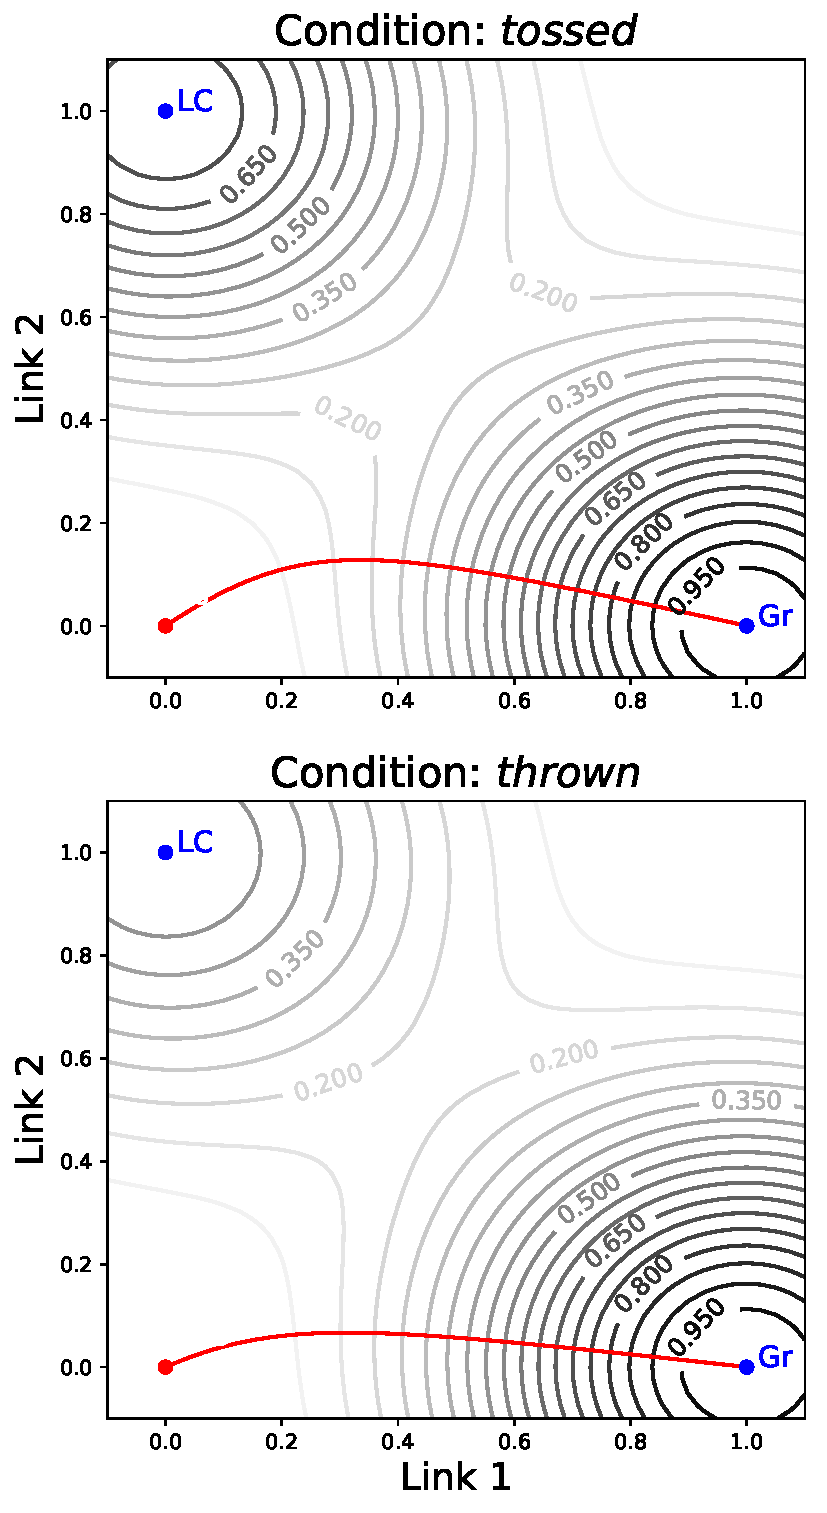
\includegraphics[width=\linewidth]{../Model/HarmonyContours.pdf}
\caption{Contour plots of the harmony landscape. Top panel: \emph{tossed} condition; bottom panel: \emph{thrown} condition. Contour labels give the harmony at that level. \textbf{To do: add in sample trajectories showing the extra bowing away from the grammatical attractor for \emph{tossed}.}}
\label{harmonylandscape}
\end{figure}

We simulated both conditions 1000 times using the Euler forward discretization with a time step of 0.01. The noise magnitude was set to 0.001, $\gamma$ was 0.25. For illustration purposes, the local harmony of the ungrammatical attractor ([0, 1]) was set to 0.75 in the \emph{tossed} condition, and in the \emph{thrown} condition to 0.5 (see below for a more systematic investigation of the effect of $\gamma$). Paralleling the human data in \citeA{tabor2004effects}, the theory above predicts that the \emph{tossed} condition should be slower than the \emph{thrown} condition on average. In both cases, the noise should bump the system towards the grammatical parse in most cases because its high harmony causes it to dominate the harmony landscape. When the noise does push the state towards the low-harmony structure, it will approach it more slowly in the \emph{thrown} condition than in the \emph{tossed} condition because of \emph{thrown}'s much lower harmony. But because this happens so rarely, the average time will be dominated by fast approaches to the grammatical attractor. The low-harmony parse for \emph{tossed} will be selected more often, so its lower harmony will pull the average settling time down as much as in the \emph{thrown} condition. Thus, the presence of a relatively high-harmony competitor for the grammatical parse will cause a competition-based slowdown.

As predicted, the system settled into the ungrammatical attractor in both cases, and it did so more frequently in the \emph{tossed} condition (14.6\% of runs) than in the \emph{thrown} condition (0.2\% of runs). This caused the average settling time to be higher for \emph{tossed} (in time steps: $M = 159.157, SD = 28.492$) than for \emph{thrown} ($M = 150.064, SD = 24.332$).

The above simulation is based on the assumption that the local harmony of the locally coherent parse is higher for \emph{tossed} than \emph{thrown}, making the former a stronger competitor than the latter. However, it is not immediately clear how to best set the $h_i$. In Fig.~\ref{fnofh1}, we plot mean settling times as a function of the harmony $h_1$ of the ungrammatical parse. We used $\gamma = 0.25$ here, but this pattern holds for a wide range of $\gamma$ values. This figure shows that there is broad range of $h_1$ values such that as long as the \emph{tossed} condition has a higher $h_1$ than the \emph{thrown} condition, we will observe local coherence effects. Thus, local coherence effects are generally predicted whenever we compare higher- and lower-harmony competitors for a grammatical parse.

Something interesting happens when $h_1$ is greater than about 0.85, though. As $h_1$ increases beyond that point, the average settling times start to drop. The bottom panel of Fig.~\ref{fnofh1} suggests why: as the competing ungrammatical parse increases in harmony, the time it takes the system to settle to it approaches that of the grammatical parse, so it no longer pushes the overall average settling time up as much. In this range of $h_1$ values, there is still a slowdown due to competition, but it is not as large as the slowdowns observed for somewhat lower-harmony competitors. In effect, the model predicts that we should observe the strongest competition-induced slowdowns when the competing structure is of moderate harmony, and that we should observe smaller-magnitude slowdowns for both very low harmony competitors, and (to a lesser extent) higher harmony competitors. This behavior is, to our knowledge, unique among models of sentence processing. We speculate that this property of SOSP might provide a new explanation for the ambiguity advantage \cite[e.g.]{traxler1998adjunct}, where ambiguous structures are sometimes read more quickly than unambiguous structures. This effect has been argued to rule out competition-based theories of parsing. Future work will explore whether this property of SOSP can indeed explain the observed effects.

\begin{figure}[h!]
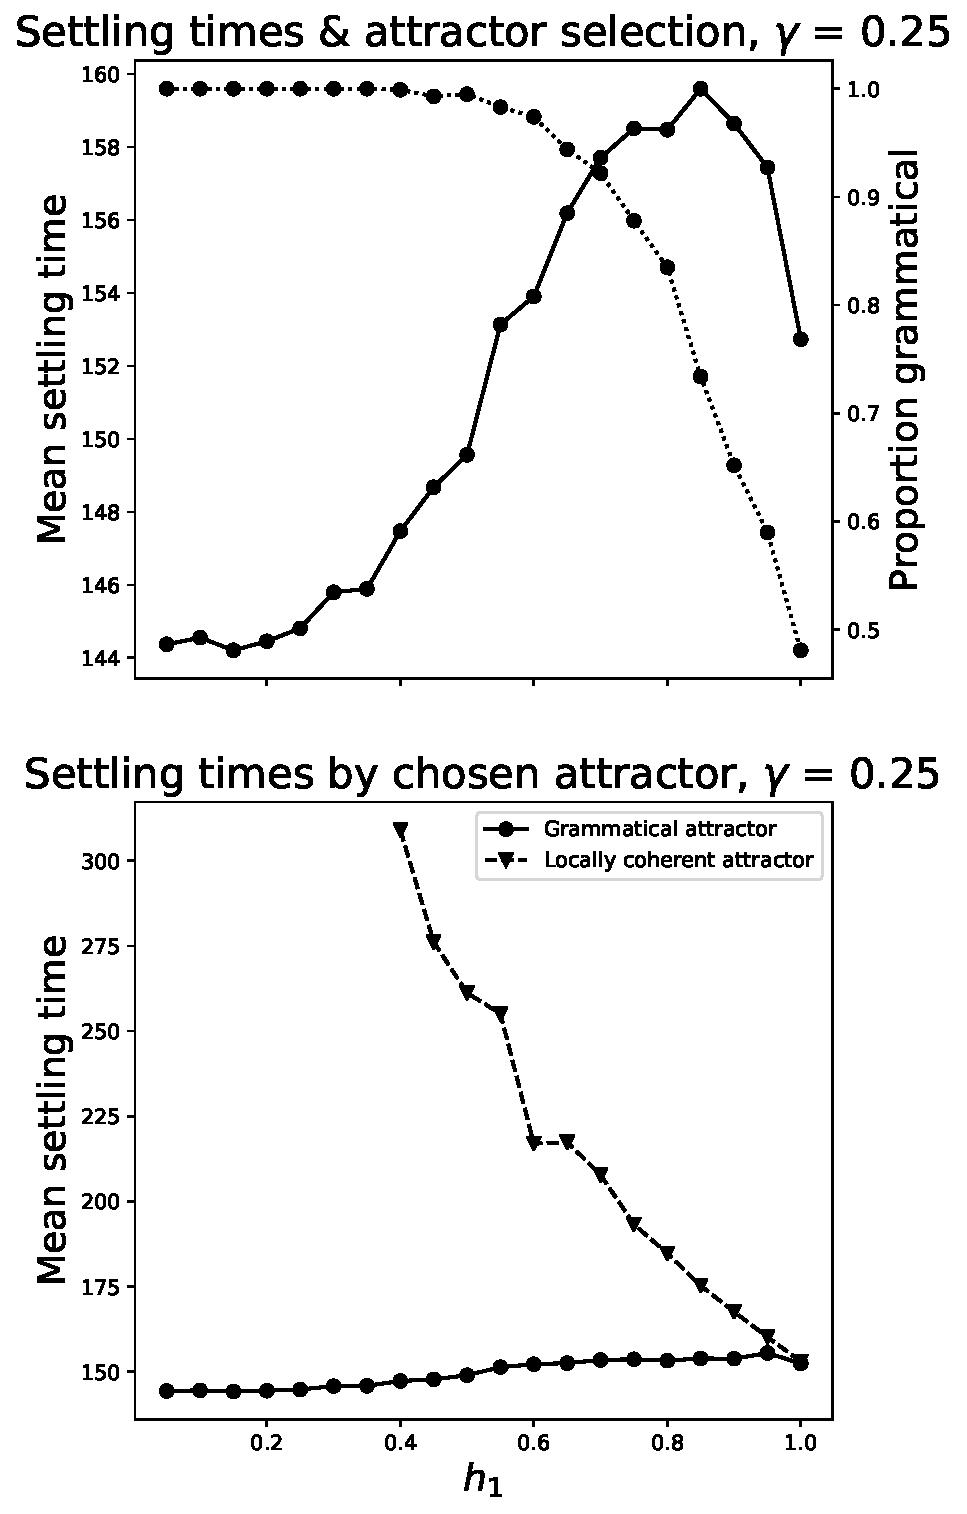
\includegraphics[width=\linewidth]{../Model/TimesAsFnOfH1.pdf}
\caption{Top panel: overall mean settling times for the local coherence model as a function of the ungrammatical parse $h_1$ (solid line, left y-axis) and the proportion of runs in which the system approached the grammatical parse (dotted line, right y-axis). Bottom panel: mean settling time broken down by chosen parse (solid line and circles = grammatical, dashed line and triangles = locally coherent parse). For $h_1 < 0.4$, the system never settled on the ungrammatical attractor. This is most likely that attractor does not exist below that point (see bifurcation discussion above).}
\label{fnofh1}
\end{figure}

\section{Discussion}
In this paper, we have introduced a theory of timing effects in a self-organizing sentence processing (SOSP) framework and demonstrated how it can explain the local coherence effects first presented in \cite{tabor2004effects}. In SOSP, the amount of time it takes to build a structure depends on how well-formed the structure is, and the average structure-building time over many trials (comparable to average reading times in a human experiment) is the weighted average of settling times to each parse chosen. We showed how this theory is derived directly from the equations of SOSP, which were designed to locally find the highest-harmony structure given the input in a harmony landscape that contains low-harmony attractors that compete with grammatical structures.

In the local coherence model, the lower-harmony attractors in the harmony landscape played a key role: when there is a relatively strong competitor for a grammatical attractor, runs in which the ungrammatical attractor is chosen increase the average settling time compared to when the competitor is even less grammatical. In this way, SOSP is different from many other theories of sentence processing that only allow the system to construct grammatical parses, e.g., surprisal calculated from probabilistic symbolic grammars \cite{levy2008expectation, hale2001probabilistic} and even Gradient Symobolic Computation (GSC; at least as it has been presented so far) \cite{cho2016bifurcation, cho2017incremental, cho2018dynamic}. The weighted averaging feature of SOSP is quite similar to recent similarity-based interference approaches building on \citeA{lewis2005} that model reading time effects as statistical hierarchical mixture models \cite{nicenboim2018models, vasishth2017feature}.

The simulations shown in Fig.~\ref{fnofh1} show that SOSP predicts local coherence effects for a broad range of parameter settings: Higher-harmony competitors will be slower than lower-harmony competitors. This prediction receives empirical support from the eye-tracking corpus study of \citeA{bicknell2009correcting}, who found widespread effects of ``single-word local coherences'' in which the probability of the part of speech tag for a word in context was highly unlikely outside that context. \textbf{Discuss noisy channel?} For very high-harmony competitors, the pattern is different, though. SOSP predicts that very high-harmony competitors will actually be faster than some medium-harmony competitors. This property might have application to the ambiguity advantage, which we leave to future research. A similar SOSP model was shown to predict subject-verb number agreement patterns in English pseudopartitives (\emph{a pile of sandwiches is/are on the table\dots}, and the SOSP framework has been argued to explain encoding interference effects in English and Italian \cite{villata2018encoding}. The present work extends the range of empirical phenomena that SOSP can explain and greatly generalizes the mathematical framework. If SOSP can indeed capture all of these effects, it would strongly support SOSP as a general theory of sentence processing.

\textbf{Add discussion of GSC}

%Discuss the relationship to Pyeong Whan's recent models. \citeA{cho2018dynamic} show that processing times in their system will be proportional to surprisal (which for them is $\Delta H$), but for us, since the input starts the system away from a (partial) parse, that this is not the same as surprisal as defined in \citeA{hale2001probabilistic, levy2008expectation}.

%Future directions: using better methods for predicting settling times, especially a way of mapping time in the model to time in actual experiments. Also, \citeA{gardiner1985handbook}, section 9.3 seems promising. In particular, long-term behavior of sys. (st. prob. distr. which is soln. of Fokker-Planck eq.) shows that the mind is vastly more likely to settle into the highest-harmony states \cite{smolensky1986information}. However, on-line processing is all about transients, where the tools are hairier mathematically...

\section{Acknowledgments}
This project was supported in part by NSF IGERT grant DGE-1144399. \textbf{others?}

\bibliographystyle{apacite}
\setlength{\bibleftmargin}{.125in}
\setlength{\bibindent}{-\bibleftmargin}
\bibliography{master}
\end{document}

%To predict how long it will take to form a particular parse, we first assume that the input or the noise has placed the state of the system in the attractor basin of that parse. We then ask how long it takes for the system to settle from that initial state $\mathbf{x}_0$ to a point close to the attractor $\mathbf{x}_1 = \mathbf{x}^* - \epsilon \cdot \mathbf{x}_0$, where $\mathbf{x}_i^*$ is the $i$th attractor and $\epsilon$ is a small constant\footnote{$\mathbf{x}_1$ therefore lies on the line connecting $\mathbf{x}^*$ and $\mathbf{x}_0$.}. This change in state will be associated with a change in harmony $\Delta H = H(\mathbf{x}_1) - H(\mathbf{x}_0)$. We follow \citeA{cho2018dynamic} in noting that it will take the system some time $t_c$ to travel this distance (and make the corresponding change in harmony), giving:
%\begin{equation}
%\begin{split}
%\Delta H &= \int_0^{t_c} \frac{dH(\mathbf{x})}{dt}dt = \int_0^{t_c} \nabla_\mathbf{x} H(\mathbf{x})^\intercal \frac{d\mathbf{x}}{dt} dt \\ &= \int_0^{t_c} \Vert \nabla_\mathbf{x} H(\mathbf{x})\Vert^2 dt = t_c \Vert \nabla_\mathbf{x} H(\mathbf{x})\Vert^2
%\end{split}
%\end{equation}
%The notation $\Vert\cdot\Vert$ is the Euclidean norm. Rearranging and evaluating $\Vert \nabla_\mathbf{x} H(\mathbf{x})\Vert^2$ at $\mathbf{x}_1$, we find that the time to get close to the attractor is:
%\begin{equation}\label{time_pred}
%t_c = \frac{\Delta H}{\Vert \nabla_\mathbf{x} H(\mathbf{x}_1)\Vert^2}
%\end{equation}
%Because we are assuming that $\mathbf{x}_0$ is already in the basin of attraction of $\mathbf{x}_i^*$, the effects of the other $\phi_j,\ j \neq i$ in $H(\mathbf{x})$ will be negligible.\footnote{As long as $\gamma$ is set small enough, $\phi_j(\mathbf{x}_1)$ will be close to zero since $\mathbf{x}_1$ will be far from the center $\mathbf{c}_j$.}. Thus, the approximation:
%\begin{equation}
%t_c \approx \frac{\Delta H}{\Vert2 h_i \gamma^{-1} (\mathbf{x}_1 - \mathbf{c}_i) \phi_i(\mathbf{x}_1)\Vert^2} \propto h_i^{-1}
%\end{equation}
%shows that the time to settle to an attractor from an initial point inside its basin of attraction will be inversely proportional to the attractor's harmony $h_i$. In this way, SOSP (and possibly other similar systems like \citeA{cho2018dynamic}) derives processing times directly from the theory of well-formedness via the processing dynamics.
%
%Each attractor will have its own $t_c$, so the average processing time for a given condition is predicted to be proportional to the average of the $t_c$ for each attractor that the system settles to in that condition weighted by the probability of settling to that attractor.


%Ignoring the effect of noise, we can calculate the time $T_i$ it takes a system to move from some initial position $\mathbf{x}_0$ to within a radius $\epsilon$ of an attractor $\mathbf{x}_i^*$ with the following equation:
%\begin{equation}
%T_i = \int dt = \int \frac{dt}{d\mathbf{x}} d\mathbf{x} = \int_{\mathbf{x}_0}^{\mathbf{x}_i^* + \mathbf{\epsilon}} \frac{d\mathbf{x}}{\nabla H(\mathbf{x})}
%\end{equation}
%This integral diverges if there is a fixed point in the interval $[\mathbf{x}_0,\ \mathbf{x}_i^* + \epsilon]$. But, if we consider that the effects of the other $\phi_j,\ j \neq i$ will be negligible as long as $\mathbf{x}_0$ is within the attractor basin of $\mathbf{x}_i^*$\footnote{As long as $\gamma$ is set small enough, $\phi_j(\mathbf{x}_0)$ will be close to zero since $\mathbf{x}_0$ will be far from the center $\mathbf{c}_j$.}, we can use the approximation:
%\begin{equation}\label{time_pred}
%\tilde{T}_i = \int_{\mathbf{x}_0}^{\mathbf{x}_i^* + \mathbf{\epsilon}} \frac{\gamma}{2h_i (\mathbf{x} - \mathbf{c}_i)\phi_i(\mathbf{x})}\ d\mathbf{x} \propto h_i^{-1}
%\end{equation}
%Thus, the time it takes to get close to a particular attractor will be approximately inversely proportional to the the local harmony of that attractor, assuming that the noise has already bumped the system into the attractor basin of $\mathbf{x}_i^*$. The average reading time in a given condition is then the average over all $\tilde{T}_i$ weighted by the probability that the system is bumped into $\mathbf{x}_i^*$'s attractor basin.
%
%\textbf{Note to Whit:} I've now realized that this approximation only works within a particular basin of attraction: if you start outside the basin of attraction for some attractor, the time diverges because the noiseless dynamics can't move against the harmony gradient. But, if we start the system in a basin of attraction and ask how long it takes to get close to the attractor, we can ensure that, when we compare between conditions, that the distance over which we integrate is equal, i.e., wherever $\mathbf{x}_i^*$ is in a given condition, we can set $\mathbf{x}_0$ to be $\mathbf{x}_i^* + \delta$, as long as $\delta$ does not put $\mathbf{x}_0$ outside the basin of attraction in either of the conditions being compared. Also, the local characteristic time scales analysis doesn't really give us any information beyond what Eq.~\ref{time_pred} does. In fact, Eq.~\ref{time_pred} is probably more important, because it doesn't assume that we're infinitesimally close to the attractor.
%
%\textbf{Second note:} The theory of average reading times relies on knowing the probabilities of settling into different parses. For in the $t \rightarrow \infty$ limit, we can easily find the stationary probability distribution over states, and we could use that when calculating average RTs, but that distribution greatly exaggerates differences in the rates of settling to particular parses (like we've discussed, a system with small noise will spend the vast majority of its time trapped in high-harmony states). Since this way would underestimate the frequency of going to a less-than-optimal parse, it would also predict very small differences in reading times between conditions. We can try this approach here, and note that it should predict the correct ordering of conditions, but the relative magnitudes would be off. A second option would estimate the probabilities by running simulations, but that weakens our attempt to make predictions directly from the equations... A third option is to not worry about the probabilities and take the $\tilde{T}_i$ as rough predictions on their own. In any case, we would be plenty to discuss for future directions...

